\documentclass[a4paper, 12pt]{article}
\usepackage{cmap}
\usepackage[warn]{mathtext}
\usepackage[T2A]{fontenc}
\usepackage[utf8]{inputenc}
\usepackage{graphicx}
\usepackage[left=30mm, top=20mm, right=20mm, bottom=20mm, footskip=10mm]{geometry}
\usepackage{amssymb}
\usepackage{amsmath}
\usepackage{wrapfig}
\usepackage{siunitx}
\graphicspath{image/}
\title{Определение главных моментов инерции твердых тел с помощью крутильных колебаний.}
\author{Шакиров Тимур Тагирович}
\date{Декабрь 2021}
\renewcommand{\figurename}{Рис.}
\begin{document}

\maketitle
\textbf{Цель работы:} Измерить периоды крутильных колебаний при различных положениях закрепленного в ней тела, проверить теоретическую зависимость между периодами крутильных колебаний тела относительно различных осей, определить моменты инерции относительно нескольких осей для каждого тела, по ним найти главные моменты инерции тел и построить эллипсоид инерции.

\vspace{1 cm}

\textbf{В работе используются:} установка для крутильных колебаний, набор твердых тел, секундомер.
\section*{Теория.}
Тензор инерции---характеристика пространственного распределения массы, определяется следующим образом:\\
\begin{pmatrix}
\rho\int\limits_V(y^2+z^2)dV& -\rho\int\limits_V xydV& -\rho\int\limits_V xzdV\\
-\rho\int\limits_V xydV& \rho\int\limits_V(x^2+z^2)dV& -\rho\int\limits_V yzdV\\
-\rho\int\limits_V xzdV& -\rho\int\limits_V yzdV& \rho\int\limits_V (x^2+y^2)\\
\end{pmatrix}\\
Правильно выбрав оси, всегда можно привести тензор к диагональному виду. Диагональные элементы $J_{x}$, $J_{y}$, $J_{z}$ при этом называют главными моментами инерции тела. У тензора есть геометрическая интерпретация---эллипсоид инерции, определяемый уравнением $J_xx^2+J_yy^2+J_zz^2=1$.\newpage
Момент инерции относительно оси, проходящей через центр масс $J=\frac{1}{r^2}$, где $r$---расстояние от центра эллипсоида до точки пересечения оси с эллипсоидом.\\
Рамка, фиксирующая положения тела относительно себя, способна совершать колебания.
$$(I+I_р)\frac{d^2\varphi}{dt^2}=-f\varphi$$
\begin{equation}
    \label{e1}
    T=2\pi\sqrt{\frac{I+I_р}{f}}
\end{equation}
\begin{wrapfigure}{l}{180pt}
    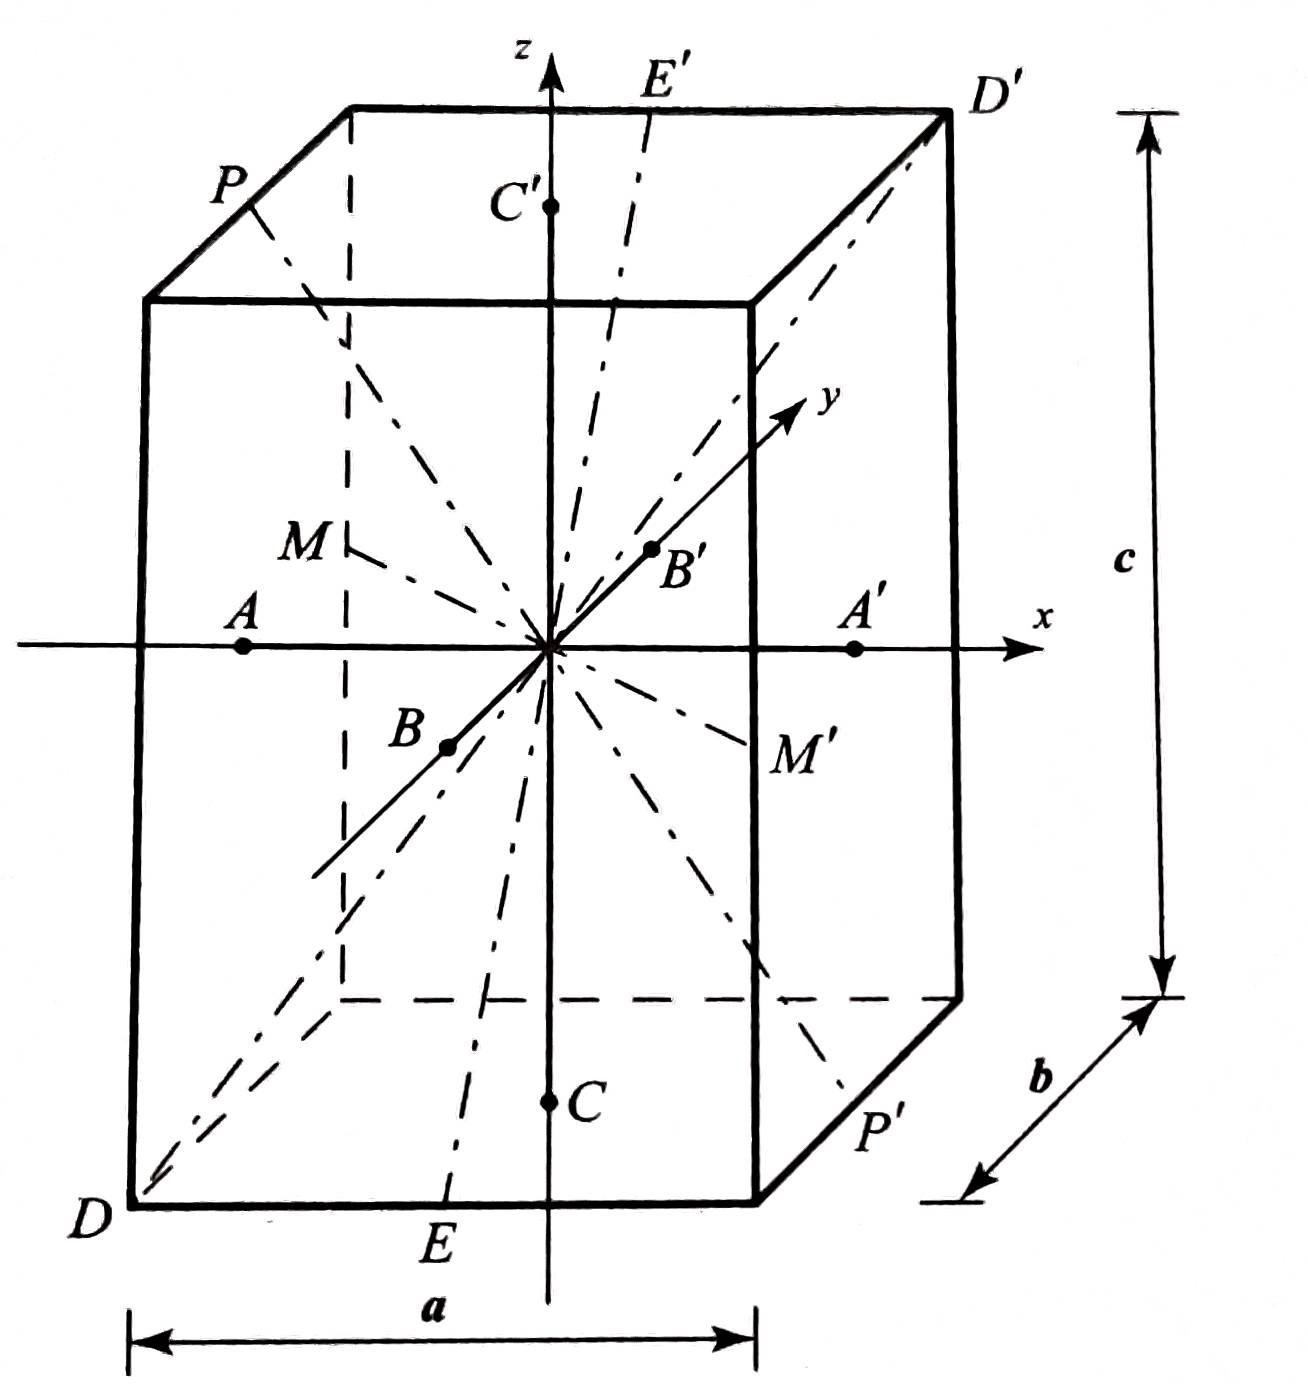
\includegraphics[width=180pt]{image/1.jpg}
    \caption{\label{p1}Оси вращения параллелепипеда}
\end{wrapfigure}
Момент инерции относительно диагонали для прямоугольного параллелепипеда: $$I_d=I_x\frac{a^2}{d^2}+I_y\frac{b^2}{d^2}+I_z\frac{c^2}{d^2}$$\\
Отсюда c учетом (\ref{e1}) получим: $$(a^2+b^2+c^2)T^2_d=a^2T^2_x+b^2T^2_y+c^2T^2_z$$
Аналогично можно получить:
$$(b^2+c^2)T^2_E=b^2T^2_y+c^2T^2_z$$
$$(a^2+c^2)T^2_P=a^2T^2_x+c^2T^2_z$$
$$(a^2+b^2)T^2_M=a^2T^2_x+b^2T^2_y$$
\vspace{10pt}
\section*{Ход работы}
\begin{enumerate}
    \item Убедились в работоспособности установки, научились закреплять в ней тела, убедились в малости затухания колебаний.
    \item Для различных тел (параллелепипед, куб, цилиндр 1, цилиндр 2, рамка 1, рамка 2) промерили периоды колебаний методом рядов для $n=10$. Также измерили геометрические размеры параллелепипеда и проверили равенства из теоретической части. Результаты внесли в таблицу:\newpage
    \begin{table}[h]
        \begin{tabular}{|c|cccc|}
        \hline \multicolumn{5}{|c|}{\textbf{Параллелепипед}}\\ \hline
        & 1& 2& 3& $T_{ср}$\\ \hline
        $T_x$, $c$& 3.88& 3.78& 3.84& 3.83\\
        $T_y$, $c$& 4.09& 4.11& 4.12& 4.11\\
        $T_z$, $c$& 3.23& 3.25& 3.22& 3.23\\
        $T_d$, $c$& 3.46& 3.48& 3.46& 3.47\\
        $T_E$, $c$& 3.34& 3.35& 3.35& 3.35\\
        $T_P$, $c$& 3.41& 3.42& 3.41& 3.41\\
        $T_M$, $c$& 3.85& 3.85& 3.84& 3.85\\
        \hline \multicolumn{5}{|c|}{\textbf{Куб}} \\ \hline
        $T_x$, $c$& 3.03& 3.06& 3.05& 3.05\\
        $T_y$, $c$& 3.06& 3.06& 3.04& 3.06\\
        $T_z$, $c$& 3.05& 3.05& 3.04& 3.05\\
        $T_d$, $c$& 3.05& 3.05& 3.04& 3.05\\
        $T_E$, $c$& 3.04& 3.07& 3.06& 3.06\\
        $T_P$, $c$& 3.06& 3.07& 3.04& 3.06\\
        $T_M$, $c$& 3.05& 3.05& 3.07& 3.06\\
        \hline \multicolumn{5}{|c|}{\textbf{Цилиндр 1}}\\ \hline
        $T_x$& 3.04& 3.08& 3.08& 3.07\\
        $T_y$& 3.26& 3.26& 3.25& 3.26\\
        \hline \multicolumn{5}{|c|}{\textbf{Рамка 1}}\\ \hline
        $T$& 2.58& 2.56& 2.56& 2.57\\
        \hline \multicolumn{5}{|c|}{\textbf{Цилиндр 2}}\\ \hline
        $T_x$& 6.80& 6.80& 6.80& 6.80\\
        $T_y$& 6.48& 6.45& 6.45& 6.46\\
        \hline \multicolumn{5}{|c|}{\textbf{Рамка 2}}\\ \hline
        $T$& 4.46& 4.44& 4.44& 4.45\\
        \hline
        \end{tabular}
        \quad
        \begin{tabular}{|c|c|}
        \hline
        $a$, $см$& 10.0\\ 
        $b$, $см$& 5.0\\
        $c$, $см$& 15.0\\ \hline
        $(a^2+b^2+c^2)T_d^2$, $см^2 \cdot с^2$&4210\\
        $a^2T^2_x+b^2T^2_y+c^2T^2_z$, $см^2 \cdot с^2$&4230\\ \hline
        $(b^2+c^2)T^2_E$, $см^2 \cdot с^2$&2800\\
        $b^2T^2_y+c^2T^2_z$, $см^2 \cdot с^2$&2770\\ \hline
        $(a^2+c^2)T^2_P$, $см^2 \cdot с^2$& 3790\\
        $a^2T^2_x+c^2T^2_z$, $см^2 \cdot с^2$&3810\\ \hline
        $(a^2+b^2)T^2_M$, $см^2 \cdot с^2$& 1860\\
        $a^2T^2_x+b^2T^2_y$, $см^2 \cdot с^2$& 1890\\
        \hline
        \end{tabular}
    \end{table}
    \item
    Для построения эллипсоидов инерции вычислим величины $\frac{1}{\sqrt{T^2-T_P^2}}$:\\
    \begin{table}[h!]
        \centering
        \begin{tabular}{|c|cccc|}
        \hline
        & параллелепипед& куб& цилиндр 1& цилиндр 2\\ \hline
        $\frac{1}{\sqrt{T_x^2-T_P^2}}$& 0.352& 0.609& 0.595& 0.194\\
        $\frac{1}{\sqrt{T_y^2-T_P^2}}$& 0.312& 0.602& 0.499& 0.214\\
        $\frac{1}{\sqrt{T_z^2-T_P^2}}$& 0.511& 0.609& &  \\ \hline
        \end{tabular}\\
    \end{table}\\
    Сечения эллипсоидов главными плоскостями прикреплены в приложении. Эксперимент подтвердил теоретические зависимости из теоретической части отчета.
\end{enumerate}\newpage
\section*{Приложение}
\begin{flushleft}
\begin{figure}[h!]
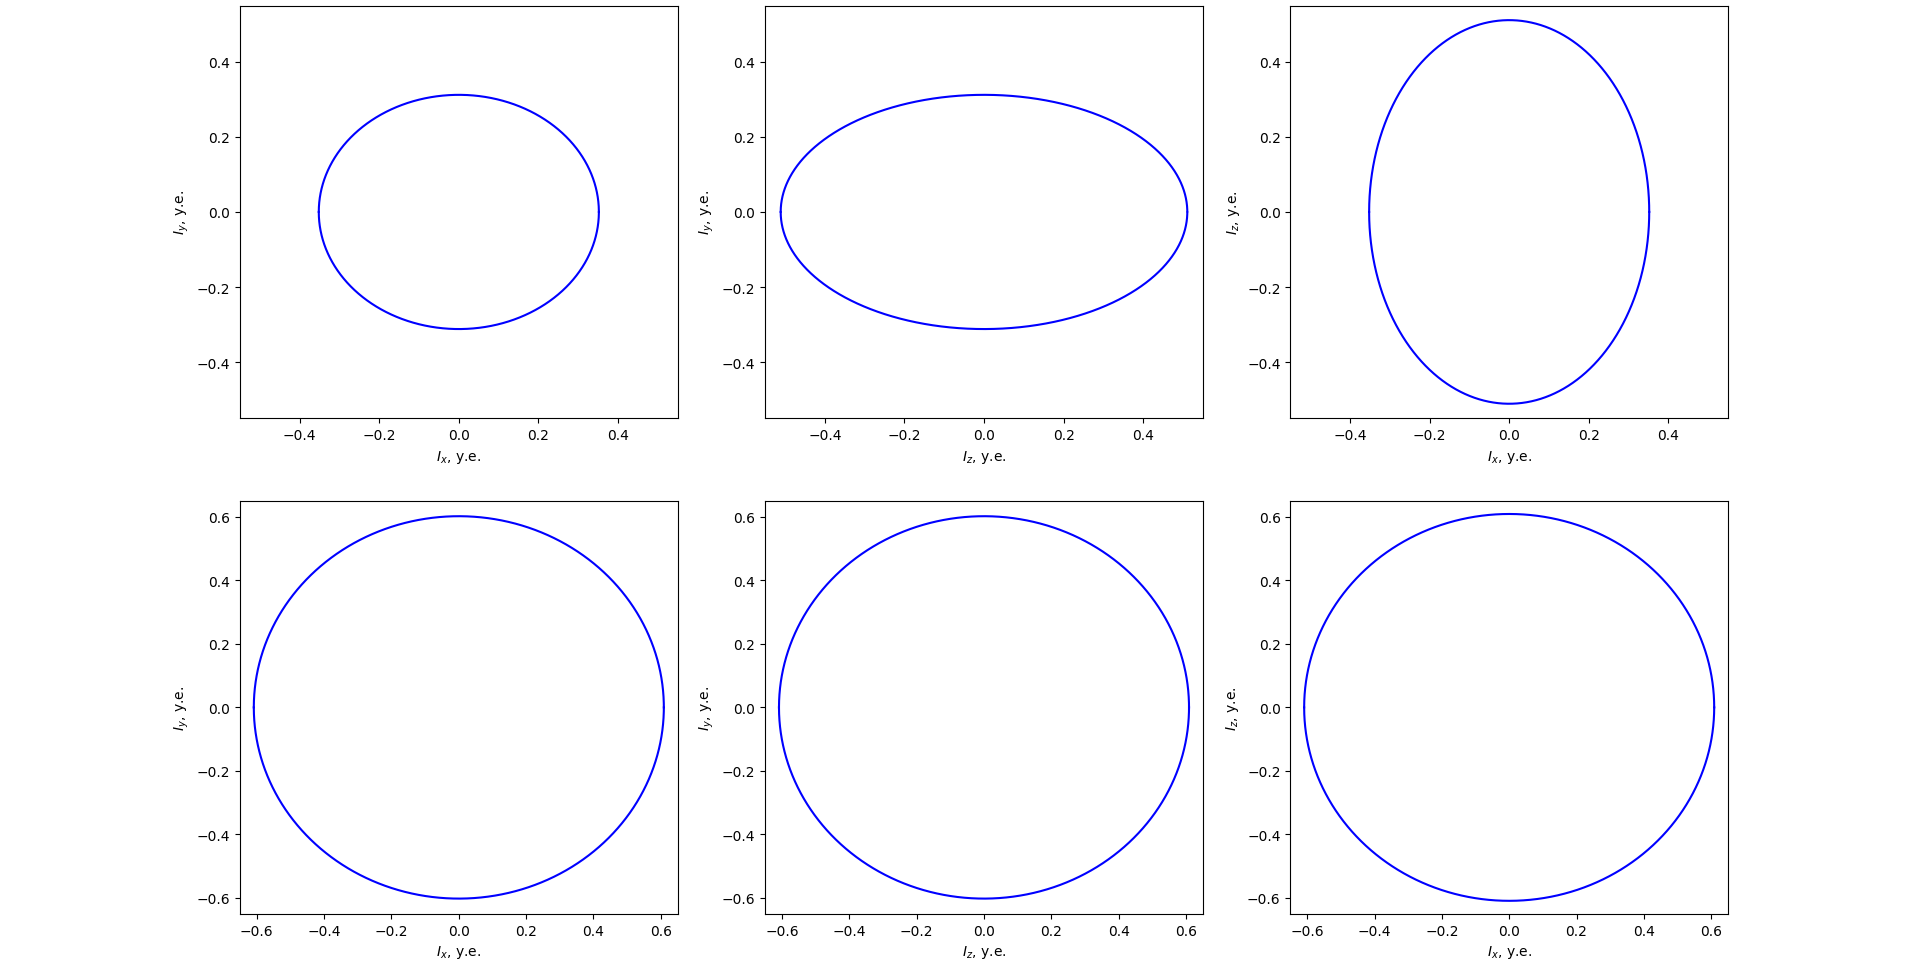
\includegraphics[width=500pt]{image/1.png}
\caption{Сечения эллипсоидов параллелепипеда(1 ряд) и куба(2 ряд)}
\end{figure}
\end{flushleft}
\begin{flushleft}
\begin{figure}[h!]
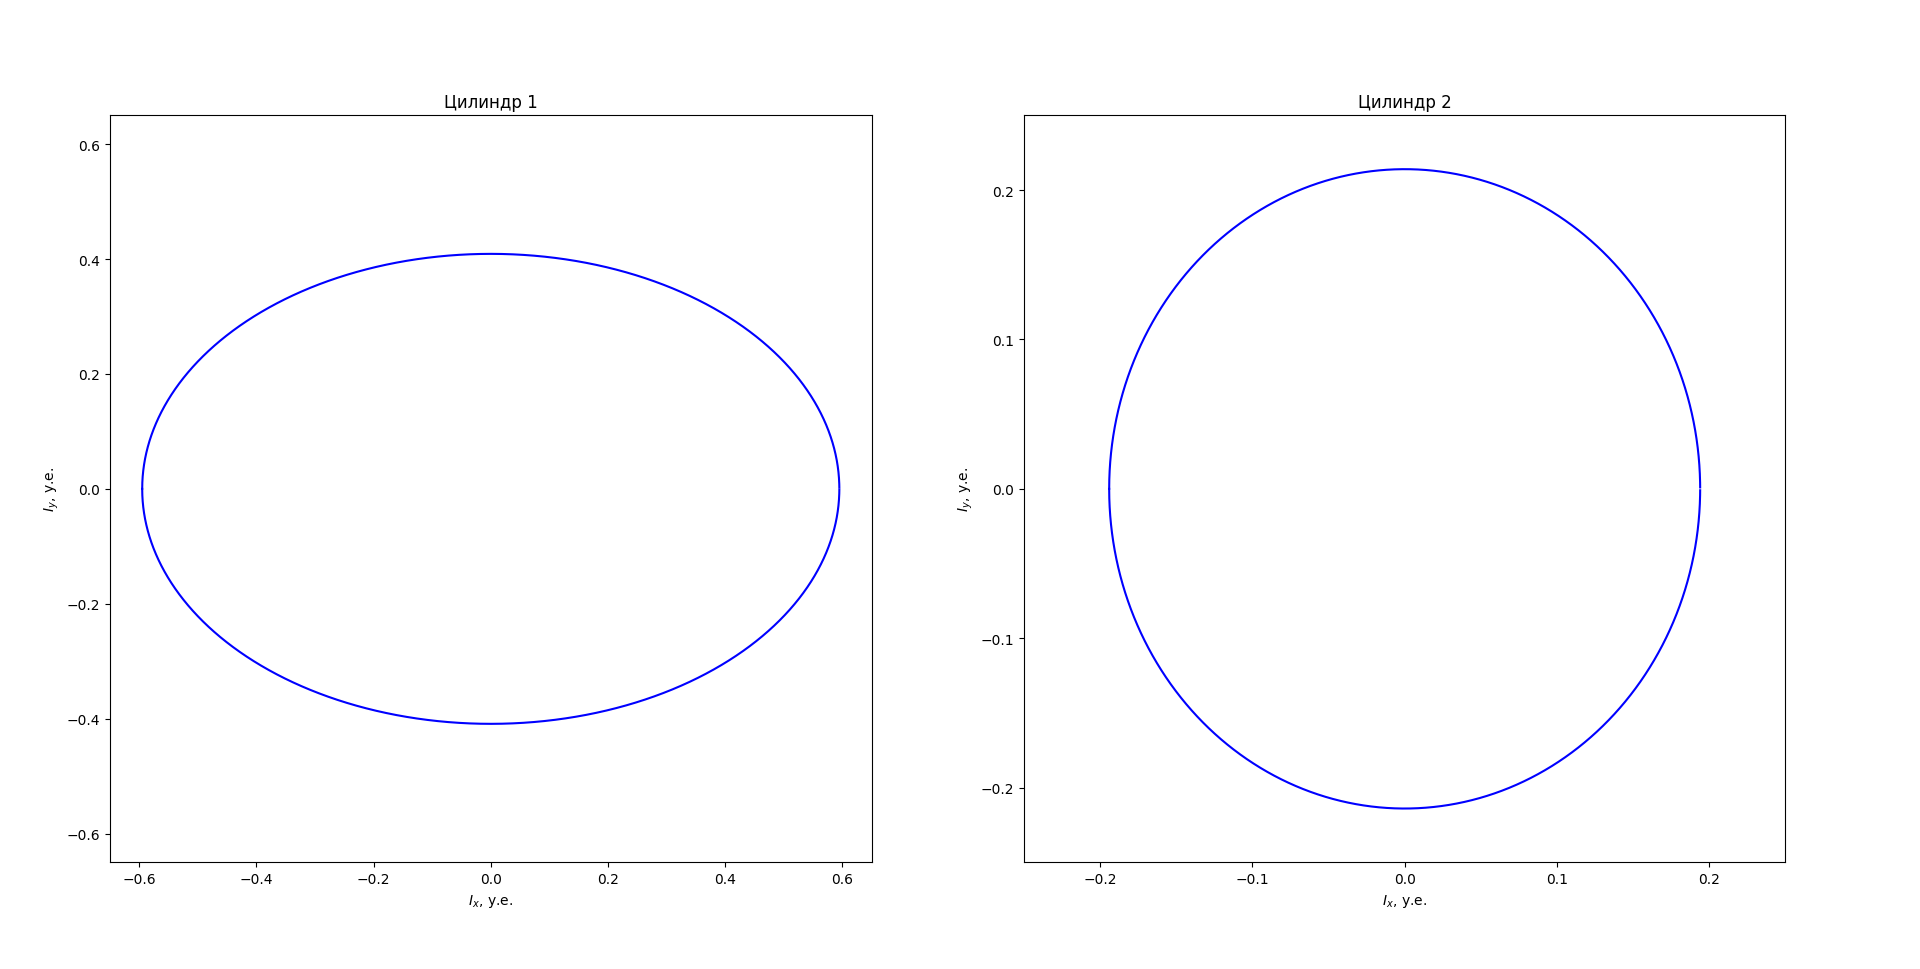
\includegraphics[width=500pt]{image/2.png}
\caption{сечения эллипсоидов цилиндра 1 и цилиндра 2}
\end{figure}
\end{flushleft}

\end{document}
